\documentclass[12pt]{article}

\usepackage{graphicx}

\usepackage[numbers,sort&compress]{natbib}

\usepackage{../phflplx/phflplx}
\DeclareGraphicsExtensions{.lplx,.pdf}

\usepackage{hyperref}

\parskip=1.5ex\relax
\parindent=0pt\relax

\begin{document}

\section{First section}

Here is my graphics:

\fboxsep=0pt\relax
\fbox{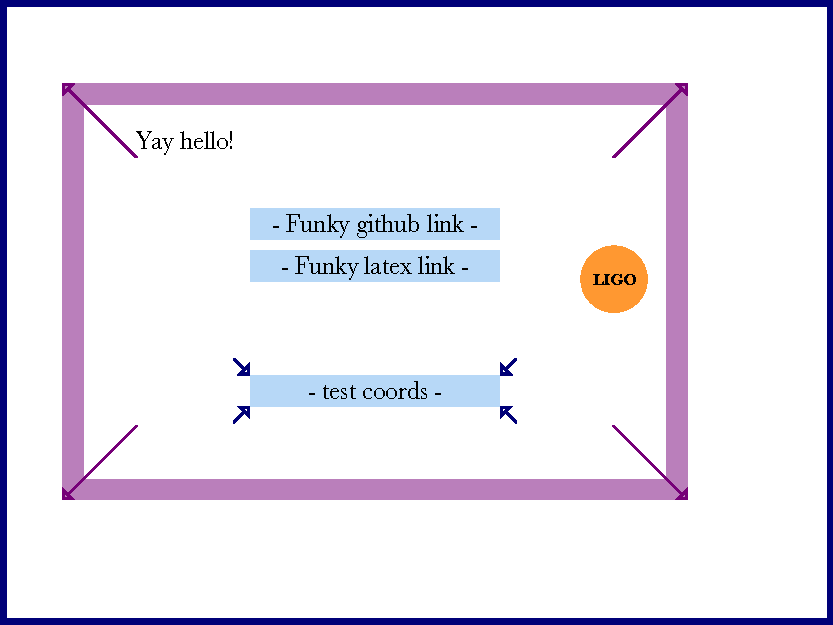
\includegraphics{testgraphics2}}

Yay!

\clearpage

Smaller: ?

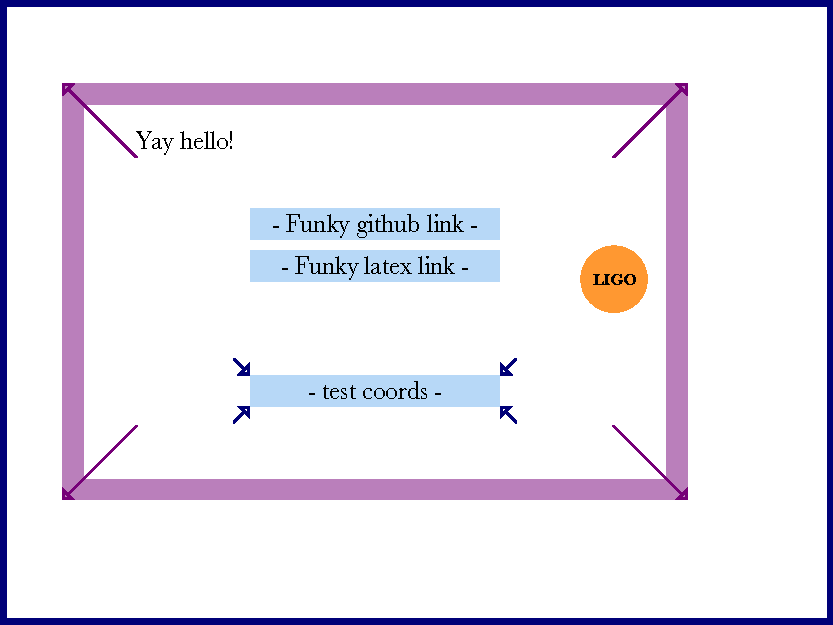
\includegraphics[width=4cm]{testgraphics2}

\vspace{4cm}
Trimmed: (but not clipped)

\fboxsep=0pt\relax
\fbox{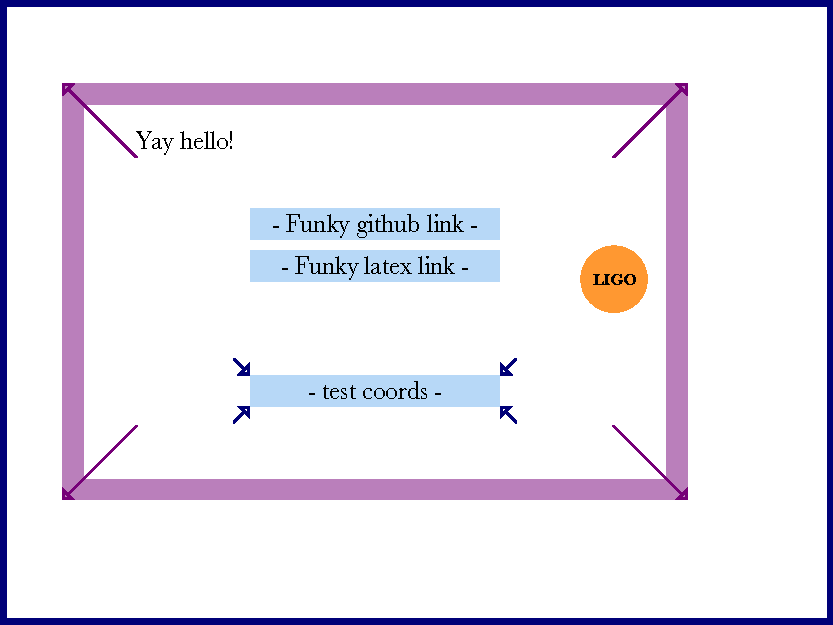
\includegraphics[trim=30pt 60pt 70pt 40pt]{testgraphics2}}

\vspace{4cm}
Trimmed \& clipped: ?

\fboxsep=0pt\relax
\fbox{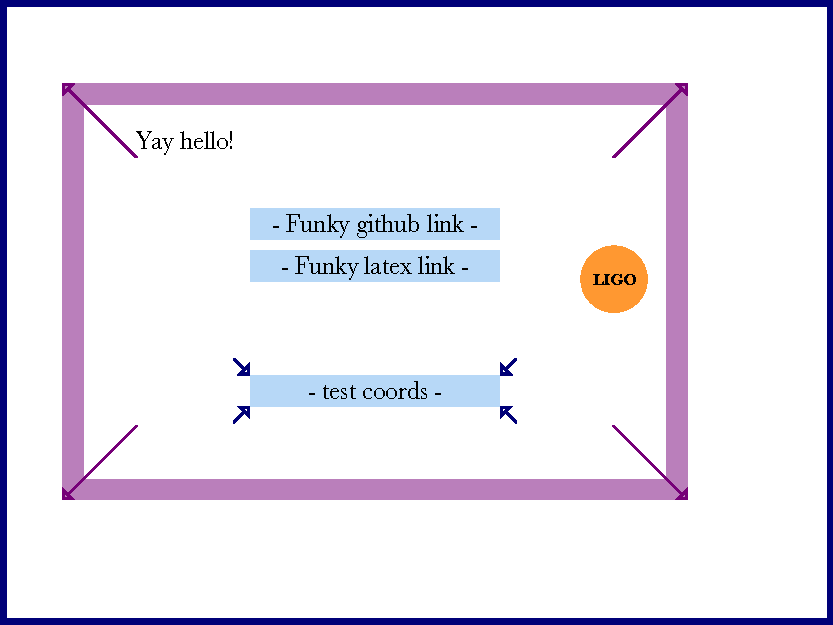
\includegraphics[trim=30pt 60pt 70pt 40pt,clip]{testgraphics2}}

\vspace{4cm}
Trimmed \& clipped with clipped links: ?

\fboxsep=0pt\relax
\fbox{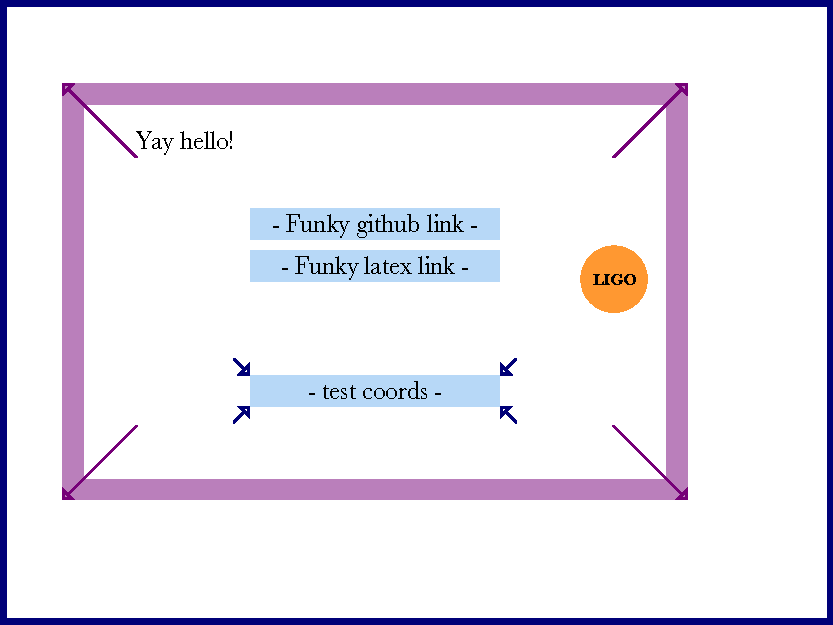
\includegraphics[trim=140pt 130pt 160pt 110pt,clip,width=200pt]{testgraphics2}}


\clearpage

Rotated \& smaller: ?

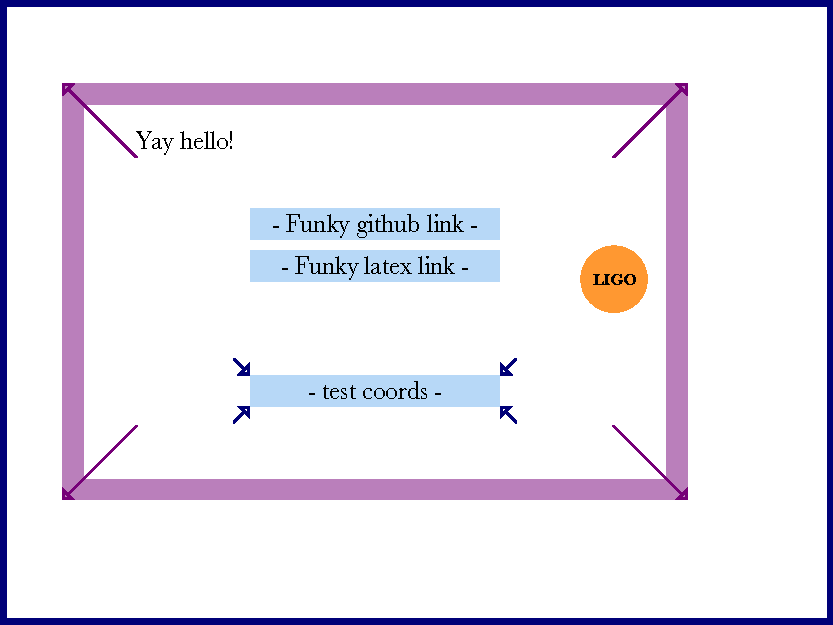
\includegraphics[angle=10,width=4cm]{testgraphics2}

Smaller \& rotated: ?

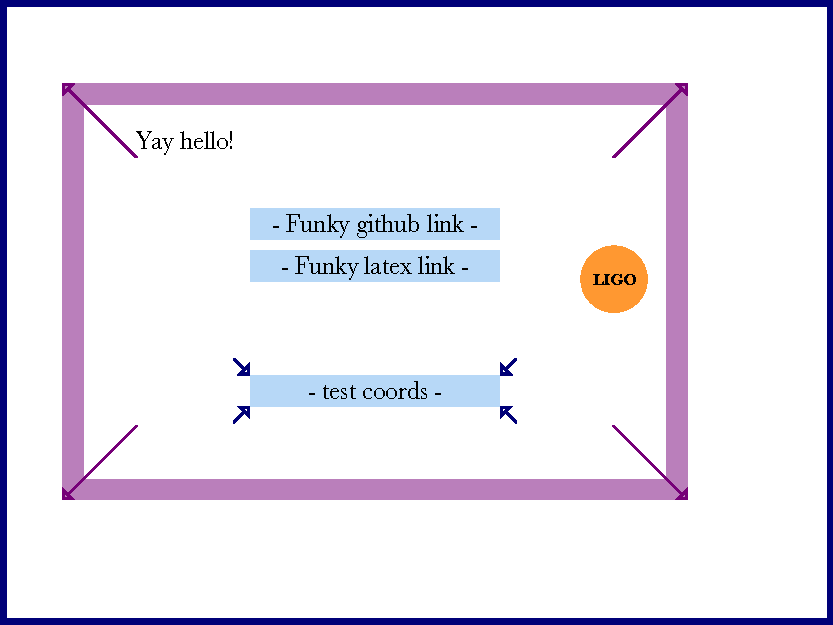
\includegraphics[width=4cm,angle=10]{testgraphics2}


\section{Test section}
\label{sec:testref}

Another section.  And also LIGO~\cite{Ligo2016} is really cool.


\begin{thebibliography}{99}
\bibitem{Ligo2016} {LIGO Scientific Collaboration and Virgo
    Collaboration.}  ``Observation of Gravitational Waves from a Binary Black
  Hole Merger,'' \emph{Physical Review Letters} {116} {061102}, {2016}.
  \\
  doi:{10.1103/PhysRevLett.116.061102}.
\end{thebibliography}


\end{document}
